\documentclass[a4paper,10pt,oneside,openright,final]{memoir} %twocolumn,
\usepackage[utf8]{inputenc}
\usepackage[russian, ukrainian, english]{babel}
\usepackage{etex}
\usepackage{times}
\DisemulatePackage{setspace}
\usepackage{setspace}
\usepackage{amssymb}
\usepackage{amsfonts}
\usepackage[pdftex]{graphicx}
%\usepackage{subfigure}
\usepackage{alltt}
\usepackage{moreverb}
%for more info on hyperref package see http://en.wikibooks.org/wiki/LaTeX/Packages/Hyperref
\usepackage[pdftex,colorlinks=true,linkcolor=blue, citecolor=magenta]{hyperref}
\usepackage{eso-pic}
\usepackage{transparent}
\setlength{\columnsep}{3em}

\usepackage{wrapfig}
\usepackage{subfig}
\usepackage{alltt}
\usepackage{moreverb}
% tikz related packages to provide scalable graphics 
\usepackage{tikz}
\usetikzlibrary{calc,mindmap,backgrounds,positioning,arrows,shapes,shapes.arrows,shapes.misc,automata,petri,patterns,scopes,chains,matrix,decorations.pathmorphing,shadows,calc}


\usepackage{geometry}
\geometry{hmargin={15mm,15mm},vmargin={15mm,20mm}}

\usepackage[pages=some]{background}

\backgroundsetup{
  scale=1.2,
  angle=0,
  opacity=0.4,
  contents={
    
\includegraphics[width=1.1\paperwidth,height=1.1\paperheight, keepaspectratio]{images/00-background.png}} 
}


%%%%%%%%%%%%% copyright %%%%%%%%%%%%%%
\title{Trident Genesis Platform}
\author{Fielden Management Services Europe LLC}
\date{}
\usepackage{hyperref}
\usepackage{hyperxmp}
\hypersetup{
    pdftitle={Trident Genesis Platform},
    pdfauthor={Fielden Management Services Europe LLC},
    pdfsubject={A hight level overview of key principles and advantages.},
    pdfcopyright={Copyright (C) 2016 by Fielden Management Services Europe LLC.  All rights reserved.}
}

\usepackage{xcolor}
\makeevenhead{headings}%
    {\thepage}{}{\slshape\bookname~\thebook\qquad\partname~\thepart\qquad\leftmark}
    \makeoddfoot{headings}{\slshape\rightmark}{\color{gray}Copyright (C) 2016 by Fielden Management Services Europe LLC.  All rights reserved.}{\thepage}
	\makeoddhead{headings}{\slshape\rightmark}{}{}


\copypagestyle{headingsnobook}{headings}
\makeevenhead{headingsnobook}{\thepage}{}{\slshape\leftmark}

\begin{document}
\maketitle

\onehalfspacing

\BgThispage

\section*{The background}

	It is a well known fact that a significant number of enterprise software systems fail while still at the development stage or fail to deliver on their promise from the business perspective.  
  	Recognising the fact that this problem has multiple causes (e.g. organisational, requirement management, skills), we would like to specifically emphasise the aspect of \emph{software construction}, which we believe has a significant influence on both the initial system development as well as the change support of the deployed systems.  
  
  	Robert Martin, who is one of the strongest proponents of the importance of software construction, stated in his speech at the NDC~2012 conference that there were no significant improvements to the processes of software construction comparing to the results in object-oriented analysis of the 1990th. 
  	In his experience, today's prevalent software development practices, tools and frameworks result in obstructing the core purpose of software systems at the code level.
  	Numerous frameworks and libraries such as web and ORM frameworks on the one hand facilitate software development by simplifying low level technical aspects, but on the other hand completely shadow the actual model and purpose of software systems.  
  	
	In fact, in talking about a software architecture, the emphasis is often placed at the level of some technology stack rather than at the level of an information system in question.
	For example, in the not so distant past we could hear a lot about a ``client-server architecture'', ``LAMP architecture'' or ``Java EE architecture''.
	Nova days, it is the ``microservices architecture'' that is at the centre of everyones' attention.
	Every decade or so brings a new ``solution'' in a form of a new technology stack, but constructing reliable enterprise software systems remains one of the most difficult problems in Software Engineering.	
	This problem is important and there is a good understanding that approaching it by trying to fix the architecture at the level of a technology stack is insufficient.

    An influential work by Ivar~Jacobson~\cite{jacobson1992} describes an approach (aka OOSE) for designing software and implementing the core business functionality as a set of use cases that are independent from any specific technology such as a web framework or some communication protocol.
  	One of the intents of this approach is to enable easy migration of the core functionality (the business value) to any new or different software technology stack.
  	However, Jacobson's approach has two limitations that are important to our discussion:
	\begin{enumerate}
   		\item The part of the core functionality that provides a way to tap into the supporting technology (so-called boundaries) significantly complicates the development process.
   		\item The use case approach limits capabilities of the application by enforcing a rigid behaviour.
  	\end{enumerate}
  
	The first limitation forces developers to keep changing implementation of boundaries whenever either the supporting technology or the core business functionality changes.
	The second limitation hides the domain model from end-users by restricting interaction between the system and end-users to the scope of predefined use cases.
	This corresponds to the \emph{conversational metaphor} as defined in~\cite{HHN1986}, which is natural for process-oriented software systems\footnote{A popularity of process orientation seems to be related to a wide spread adoption of the imperative programming paradigm that heavily influences the overall design of software systems, including UI.}.

	Hiding the underlying business model complicates reasoning about a software system for both the users and the developers.
	This impedes communication between different stakeholders.  
	The \emph{world model metaphor}~\cite{HHN1986} emphasises the importance of a transparent representation of the business model at the User Interface (UI) level.
	This way users can directly interact with the model without any intermediate representations.
  	The application of the world model metaphor to the system design has been researched by Richard Pawson~\cite{pawson2001, pawson2004}.
  	His research resulted in creation of architectural pattern \emph{Naked Objects} and a framework of the same name.
  	The Naked Objects pattern reinforces the MVC pattern by promoting domain-oriented style for capturing the business model (M) and supporting an automatic generation of UI (VC) from that model.
  	By employing domain-orientation for modelling, Naked Objects falls into the category of domain-driven design~\cite{haywood2009} that provides an alternative to Jacobson's approach for system design~\cite{evans2003, vernon2013}.
    
    This pattern has its many shortcomings, but the core ideas behind it, such as \emph{world model metaphor} and the \emph{direct manipulation principle}, resonated with our understanding of how to approach the problem of designing and constructing reliable enterprise software.
        
    
\section*{Introduction}
    
	Trident Genesis (\texttt{TG}) is a software development technology for constructing highly maintainable information systems that model complex business domains\footnote{The complexity of a business domain is defined as the number and nature of interdependencies between different domain entities and properties within any individual entity.}.
	It has been created out of internal needs for our company to reduce the technical complexity, increase reliability and improve maintainability of our software, which represents a range of ERP/EAM systems.
	These include information systems for a variety of industries such as Air Traffic and Navigation Services, Rolling Stock, Chemical Industry, Fleet and Ambulance Services.
	There is an inherent complexity\footnote{As opposed to accidental.} in such systems due to the real world complexity of the equipment, assets and other physical or virtual artifacts that are used in those industries as well as complex interdependent business rules that govern them, such as safety and competency regulations, preventive maintenance cycles, inventory reordering, financial rules, plant shutdowns, temporal availability profiles etc.
	
	Effective communication between all stakeholders is a key in achieving the necessary goals in any undertaking. 
	That is why we view an information system as a communication tool that should facilitate cooperation between all participants. 
	Property constructed system should facilitate cooperation between users, their cooperation with the developers of the system and the cooperation within the development team itself.
	In order to achieve this, a technology for constructing information systems should have an appropriate representation or abstraction that would support communication and a ubiquitous language~\cite{evans2003} that shared by all stakeholders\footnote{This should be thought of as a well established terminology in a specific business domain.}.
	\texttt{TG} establishes such an abstraction in a form of an architectural pattern to model the business domain and to construct the User Interface that follows a \emph{direct manipulation} principle~\cite{shneiderman1982, shneiderman1983}.
	The latter represents the underlying domain model transparently, providing a way for users to directly interact with it.

	The developed architectural pattern is unique in approaching the design of information systems from the perspective of the their three essential functions~\cite{oli2007}:
	\begin{enumerate}
    	\item \emph{Memory}: to maintain a representation of the state of a domain.
    	\item \emph{Informative}: to provide information about the state of a domain.
    	\item \emph{Active}: to perform actions that change the state of a domain. 
	\end{enumerate}  	
	In \texttt{TG} all these functions are modelled uniformly by consistently utilising the same programming primitives.
	This ensures structural consistency for all parts of the system, which makes it ideal for iterative development and later changes during the production lifecycle of a system.
		
	An information systems that is developed with \texttt{TG} is an object-oriented construct with a responsive HTML5 front-end, which supports desktop and mobile profiles, a relational database system for state persistence and an application server that is build on RESTful principles and can be easily scaled with technologies such as Docker and load balancing.
	
	We have developed \texttt{TG} for our own needs and successfully used it to provide our customers with better, more reliable software, which is used in mission critical operations.
	Our team of Delphi developers, who were accustomed to a very procedural, UI driven approach, was successfully trained to shift their thinking away from low level technical details and approach software development from a business domain modelling perspective, which is fostered by \texttt{TG}.
	Once foreign, the practice of domain-driven unit testing to validate the business model and rules became a part of normal day-to-day software construction routine.
	
	
	The following sections delve more into details about TG.
	This includes the discussion of the developed architectural pattern and the influence of the REST architectural style on the modelling at the level of objects; how is it used to ensure a uniform model of an information system and how does it satisfy the SOLID principles; why controlled mutation it important and how immutability helps prevent accidental mistakes; how unit testing becomes domain-driven and why business processes could benefit from becoming persistent.
	We also discuss the Entity Query Language for simple and non-trivial data querying and how the direct manipulation principle is employed for building consistent and intuitive user interfaces.
	This overview is concluded with a brief discussion of a fairly sophisticated information systems that is utilised in mission critical operations by one of our customers in the domain of Air Traffic and Navigation Services.

\section*{The problem statement}

	It puts the modelling of a business domain in the centre of software requirement management, design and construction by following a very specific architectural pattern called \emph{Fractal Objects}.
	The unique trait of the \emph{Fractal Objects} pattern is in establishing a uniform approach for designing and implementing the three core functions of any information system~-- memory, informative, active~\cite{oli2007}.
	This results in a holistic system design and implementation that is maintainable and of high fidelity with the target business domain.

	The current definition and functions of an information system was defined back in 1970s.
	

	
	There are two metaphors in the context of information systems construction -- conversational and world model.
	They convey the meaning of two very different principles that underpin an information system -- both with their cons and pros.
	
	More traditional, but now again in the centre of everyones' attention due to the raise of micro services, is the conversational metaphor.
	Information systems that follow it, do not permit a direct interaction of users with an underlying data model.
	Instead, a UI and API layers act as an intermediary, hiding the underlying model of an information system.
	
	The world model metaphor emphasises the direct manipulation principle where users query and change the data by interacting with the underlying model.
	
	Any data model can be viewed as a pair of languages -- a language for describing the data and a language for interacting with it.
	For example, in relational databases, the Data Definition Language (DDL) is used to describe the data and the Structured Query Language (SQL) is used to interact with it.
	A data model is central to any information system.
	Thus, the pair of languages is for defining and interacting with the data is of the essence.



\section*{What is Trident Genesis?}
  Trident Genesis (TG) is an opinionated software platform for developing business applications in a domain driven way.
  It lifts the level of abstraction up to the modelling of the business domain, while automatically handling low level technical details.
  
  \vspace{3 mm}
  \noindent The architecture of the business domain is often unique. 
  This is what makes companies competitive.
  Capturing the business domain model in a form of a functional software system that facilitates business operations represents the core value for customers.
  
  \vspace{3 mm}
  \noindent The TG platform incorporates over 30 years of experience in delivering Enterprise grade software solutions at a software architecture level.
  It encapsulates the complexity of the low technical details for efficient database communication, concurrent data processing, HTML5 client construction enabling software developers to concentrate on the business domain architecture.

\begin{figure}[!h]
    \vspace{-5pt} 
    \centering    
    \begin{tikzpicture}[node distance=1cm, auto, opacity=0.8, scale=0.7, every node/.style={scale=0.7}]
      \tikzset{
	  mynode/.style={rectangle,rounded corners,draw=black, top color=white, bottom color=blue!50,very thick, inner sep=1em, minimum size=3em, text centered, text=blue!50!black},
	  platform/.style={rectangle,rounded corners,draw=black, top color=white, bottom color=green!50!white,very thick, inner sep=1em, minimum size=3em, text centered, text=green!50!black}
      }  
      \node at (1, 1) [mynode] (ap1) {Application};
      \node at (1.7, 1.7) [mynode] (ap1) {Application};
      \node at (2.4, 2.4) [mynode] (ap1) {Application};

      \def\platformpath{-- +(5cm,0cm) -- +(5cm,2cm) -- +(3cm,2cm) -- +(3cm,2.5cm) -- +(4cm,2.5cm) -- +(2.5cm,3.5cm) -- +(1cm,2.5cm) -- +(2cm,2.5cm) -- +(2cm,2cm) -- +(0cm,2cm) -- cycle}
      \draw (-1,-3.3) [platform] \platformpath 
	    node [below,text width=7em, text centered,xshift=2.2cm,yshift=0.8cm] {Trident Genesis Platform};  
    \end{tikzpicture}
    \vspace{0pt} 
  \end{figure}

  \noindent The typical software construction workflow with TG encompasses: modelling of the business domain (declarative ontological aspect), implementing core business rules (imperative aspect) and configuring the user interface.
  These steps are facilitated by high level abstractions provided by the platform.
  The platform enables developers to concentrate on the modelling of the business domain. 
  This ensures higher productivity, quality and value of the final software system for the business.


 \subsection*{Principles and Advantages}
  	TG is designed to ensure that the application facilitates communication between different business stakeholders and is easy to use by incorporating the following principles and approaches.

\subsection*{Unique object-oriented architectural style to uniform modelling of the business domain}
	One could argue that commanding a programming language is relatively easy. 
  	However, object-oriented design is a different story.
  	It takes many years to become an experienced software architect.
  	TG provides a well defined architectural style that not only solves low technical tasks, but most importantly incorporates a unique architectural approach to uniform modelling of the business domain.
  	The platform ensures that all TG-based applications follow exactly the same development and modelling style, which leads to structural and behavioural uniformity of the final software system.
  	This protects developers from a multitude of programming errors.
	It enables agile development of working solutions that can be easily supported by both the original or new developers.

    \begin{figure}[!h]
    %\vspace{20pt}
    \centering    
    \begin{tikzpicture}[>=latex', scale=1.0, every node/.style={scale=1.0}]
      \tikzset{
	  outercore/.style={circle, fill=blue!50!white, inner sep=0em, minimum size=0.6cm},
	  core/.style={circle, shade, ball color=green!50!white, inner sep=0em, minimum size=0.3cm},
	  score/.style={circle, fill=green!50!black, inner sep=0em, minimum size=0.3cm},
	  outer/.style={circle, fill=blue!50!white, inner sep=0em, minimum size=2.3cm},
      }
      \begin{scope}[opacity=0.8]
	\node (o) at (0, -0.25) [outer, opacity=0.3] {};      
	\fill[circle, color=green!50!white] (0, -0.25) circle (0.7cm) node [below,text=blue!50!black,yshift=1.1cm] {Synthesised Domain Entity Model};
      \end{scope}
      
      \begin{scope}[scale=0.3,opacity=0.8]
	\node (t) at (0,0) [outercore, opacity=0.5] {};	
	\node at (0,0) [core, opacity=0.5] {};

	\node (r) at (1,-1.2) [outercore, opacity=0.5] {};	
	\node at (1,-1.2) [core, opacity=0.5] {};

	\node (l) at (-1,-1.2) [outercore, opacity=0.5] {};	
	\node at (-1,-1.2) [score] {};
      \end{scope}
      
      \node (pe) at (1.3, 1.5) [text=green!50!black,scale=0.8] {Persistent Entities};      
      \fill [green!50!black,->,out=-100, in=80] (pe.south) edge (t.north);
      \fill [green!50!black,->,out=-100,in=80] (pe.south) edge (r.north);
      
      \node (se) at (-1.3, 2) [text=blue!50!black,scale=0.8] {Synthesised Entities};
      \fill [blue!50!black,->,out=-60,in=160] (se.south) edge (l.west);
      \fill [blue!50!black,->,out=-80,in=160] (se.south) edge (o.west);      
    \end{tikzpicture} 
    \vspace{-60pt}
  \end{figure}

\subsection*{Single programming language (Java)}
	Modern software technology stacks are diverse and complex.
	Separate layers often follow different approaches, and may require different languages to use them.
	Databases require SQL knowledge, constructing Web UI requires the knowledge of HTML, CSS and JavaScript, the middleware requires some other language such as Java, Scala or C\# as well as associated frameworks.
	All of this makes software construction a complex multidisciplinary activity.
	Adding the requirement for proper modelling of the actual business domain on top of that only complicates the situation, which explains why so many software projects do not get completed or fail under their own weight during the maintenance lifecycle.
	That's why one of the core principles of TG is \emph{one language to rule them all}.
	This single language is Java, one of the currently most popular programming languages.
	Application developers that know Java can use TG to concentrate on building a core business value and deliver scalable and responsive software solutions without delving deep into the underlying technology stack.
	The developers continue to use their favourite IDE and take advantage of interactive debugging and static code analysis tools.

\subsection*{Optimised for relational databases}
	The TG platform was developed inside-out -- this is the solution we use to deliver high quality EAM/ERP systems to our customers.
	That's why unlike alternative solutions that follow the hype of NoSQL and Object-Relational databases, the TG platform provides optimised integration with relational databases such as Oracle, SQL Server and PostgreSQL.
	It utilises the business domain knowledge from the model in order to dynamically optimise queries and adjust to data usage patterns at runtime.
	Instead of using SQL, which does not fit well into the object-oriented thinking, the platform provides Entity Query Language, which is an embedded domain specific language that allows expressing data queries in a natural manner for object-oriented models by traversing the object graph.

\subsection*{Automated business domain model verification by means of domain driven testing}
	The notion of automated testing is frequently used to ensure the quality of software systems.
	Unfortunately, often unit and functional testing is an afterthought and software technology stacks need to be expanded with additional facilities to enable such testing, and these do not necessarily fit well with the rest of the layers.
	The TG platform provides first-class support for unit and functional testing in a domain driven way.
	Tests get specified against the developed business domain model by using that model.
	Unit and functional tests represent verification rules and the provided domain driven testing approach ensures their evolution alongside the underlying business domain model.
	This makes Test Driven Development (TDD) a natural approach to developing software systems with TG.
	
\subsection*{Continuous validation and integration of the business domain models during the system lifecycle}
	The TG platform stands on the shoulders of giants.
	This is no different when it comes to continuous integration (CI) and validation of TG-based software systems.
	The domain driven testing is fully compatible with modern CI tools like Jenkins and Hudson.
	Thus, the systems lifecycle can be fully integrated with one of CI tools to ensure continuous validation of the business domain model underpinning the software system.

\subsection*{Direct interaction and manipulation of the business domain model}
	The world model metaphor is fundamental to the TG platform, where the \emph{world} is an actual business domain model.
	This means that software developers and the end system users have direct access to the same model!
	While developers interact with the model at the code level and can enhance it, the system users can interact with and manipulate exactly the same model through UI.
	Users can review business entities, their relationships, enhance them with calculated properties from UI for the purpose of data interrogation, analysis and reporting.
	This significantly reduces the misconceptions about the system's actions, structure and logic, and empowers the users to truly utilise the capabilities of the business domain model to its fullest potential.
	Instead of using external tools for accessing raw data in underlying databases, the users are provided with an embedded business intelligence capability to interact with the data through a well defined business domain model.
	\begin{figure}[!h]
  		\centering
  		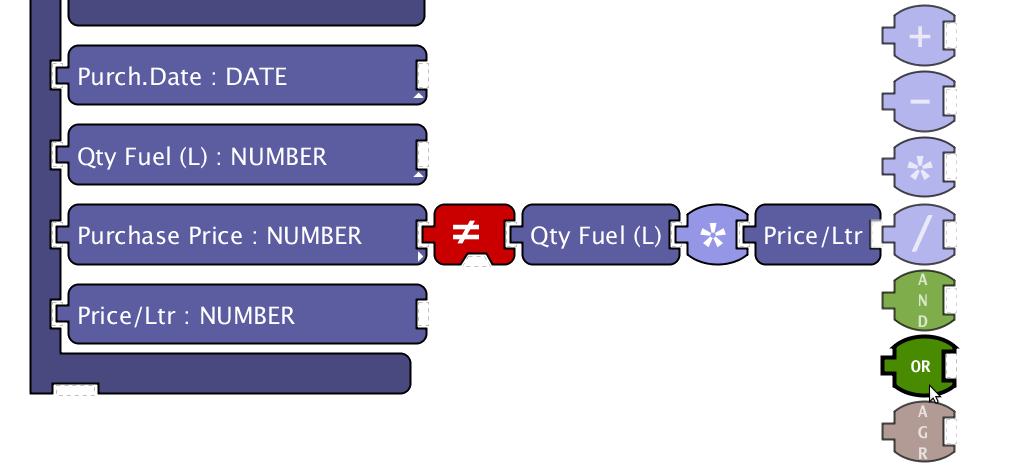
\includegraphics[scale=0.20]{images/01-rulesarea-suggestionmenu.png}  
		\vspace{-30pt} 
  	\end{figure}

	\BgThispage
\subsection*{Responsive HTML5 clients}
	TG employs an internal domain specific language for defining responsive Web UI.
	The UI concepts are all based on the business domain modelling principles to reinforce the world model metaphor, and follow the Google Material Design spec to deliver responsive and consistent User Experience (UX) across devices of multiple form factors.
	The TG presentation layer is based on Web Components (built with Google Polymer), which enables reuse and integration of in-house and $3^{rd}$ party components.
	TG offers a search-first approach to UX design that provides users with sophisticated first-class data retrieval tools supporting model-driven selection criteria, value autocompletion, ranges, meta-conditions (e.g. missing value, this year, previous fortnight), aggregations and sorting of the result sets. 

	
\subsection*{A software construction tool to facilitate the process management}
	Agile, Kanban, Scrum, FDD, TDD\ldots all of these and more are the management techniques, methodologies and methods to ensure the development of high quality and timely delivered software systems.
	These project management approaches exist for a good reason and there are multiple tools that assist with their implementation and practicing.
	This, however, is only one side of the coin.
	Implementing a proper process management method does not solve the software construction problem.
	It does not take away the technical needs and issues that arise during software construction.
	It can only help in mitigating them.
	That's why having an appropriate software construction tool that works well together with the process management method is vital to the success of any software project.
	Using the TG platform elevates software developers to the business domain level, establishes a ubiquitous business domain specific language to facilitate communication between the project stakeholders.


\subsection*{Robust Security}
	Industrial grade security, which includes HTTPS communication, the use of a key stretching PBKDF2 based password hashing, mutating session authenticator strategy, reduced sign-on with the support of both trusted and untrusted devices. 
	Support for multi-factor authentication scheme. 
	Declarative authorisation with pluggable backends (e.g. LDAP).

    
    
\subsection*{Cloud ready}
	Software systems built with TG are cloud ready.
	The platform employs RESTful architecture to structure application web-resources.
	This ensures clean separation between different business domain boundaries, UI resources and provides excellent capacity for scalability.

\subsection*{Complete application development lifecycle}
	One of the key meta-features of the Trident Genesis platform is its ability to support a complete lifecycle for developing software systems.
	This was one of our essential goals.
	Otherwise, there would always be low level technical aspects to software development that interrupt high level business domain oriented developer thinking.
	Thus, the development of software systems with TG covers all that is required for end-to-end software construction.
	This includes orthogonal aspects such as unit and functional testing, build and installation, business model design and database integration, UI definitions, secure HTTP communication, scalability and more.


%
% ---- Bibliography ----
%
\begin{thebibliography}{5}

\bibitem{Barnes:2007:ORM}
Bar\-nes, J.~M. Object-Relational Mapping as a Persistence Mechanism for Object-Oriented Applications, 2007,
\href{http://digitalcommons.macalester.edu/mathcs_honors/6/}{Online}

\bibitem{DeMichiel:2012:JPA}
De\-Mi\-chiel. L. JSR 338: Java Persistence API, Version 2.1, 2012,
\href{http://jcp.org/aboutJava/communityprocess/pr/jsr338/index.html}{Online}

\bibitem{evans2003}
Evans, E. Domain-Driven Design: Tackling Complexity in the Heart of Software, 2003, Addison-Wesley Professional.

\bibitem{Fowler:2010:DSL}
Fow\-ler, M. Domain-Specific Languages, Addison-Wesley Professional, 2010.

\bibitem{Fowler:2012:OH}
Fow\-ler. M. OrmHate, 2012,
\href{http://martinfowler.com/bliki/OrmHate.html}{Online}

\bibitem{Fielding2000}
Fielding, R. T. Architectural styles and the design of network-based software architectures: Phd thesis, University of California, Irvine, USA, 2000.

\bibitem{HBBPB:2008}
Hambrick, G. et al. Persistence in the Enterprise: A Guide to Persistence Technologies, 2008, IBM Press.

\bibitem{haywood2009}
Haywood, D. Domain-Driven Design Using Naked Objects, 2009, Pragmatic Bookshelf.

\bibitem{Hodych:2012}
Hodych, O. et al. Visual Domain-Specific Query Language for Business Applications, in Proceedings of 14-th International Conference on System Analysis and Information Technologies (SAIT 2012), Kyiv, Ukraine, 2012, pp. 311-312.

\bibitem{Hodych:2013}
Hodych, O. et al. Object-relational mapping: Limitations of data querying, in Proceedings of 15-th International Conference on System Analysis and Information Technologies (SAIT 2013), Kyiv, Ukraine, May 27-31, 2013. — P. 376–377.

\bibitem{HHN1986}
Hutchins, E., Holland, J. and Norman, D. Direct Manipulation Interfaces, in User Centered System Design: New Perspectives on Human-computer Interaction, 1986, CRC Press.

\bibitem{jacobson1992}
Jacobson, I. Object Oriented Software Engineering: A Use Case Driven Approach, 1992, Addison-Wesley Professional.

\bibitem{kal1983}
Kalinichenko, L. A. Methods and tools for integrating heterogeneous databases, 1983, Nauka (in Russian).
\foreignlanguage{russian}{Original title: Калиниченко Л. А. Методы и средства интеграции неоднородных баз данных, 1983, Наука.}

\bibitem{UBob:2002}
Martin, R.~C. Agile Software Development, Principles, Patterns, and Practices, 2002, Prentice Hall.

\bibitem{Neward:2006:VCS}
New\-ard. T. The Vietnam of Computer Science, 2006,
\href{http://blogs.tedneward.com/2006/06/26/The+Vietnam+Of+Computer+Science.aspx}{Online}

\bibitem{oli2007}
Oliv\'{e}, A. Conceptual Modeling of Information Systems, 2007, Springer.

\bibitem{pawson2001}
Pawson, R. and Matthews, R. Naked objects: a technique for designing more expressive systems, SIGPLAN Notices, V.36(12), pp.61--67, 2001.

\bibitem{pawson2004}
Pawson, R., Naked Objects, Ph.D Thesis, 2004, Trinity College, Dublin, Ireland.

\bibitem{vernon2013}
Vernon, V. Implementing Domain-Driven Design, 2013, Addison-Wesley Professional.

\bibitem{shneiderman1982}
Shneiderman, B. The future of interactive systems and the emergence of direct manipulation. Behaviour and Information Technology, 1(3):237–256, 1982.

\bibitem{shneiderman1983}
Shneiderman, B. Direct manipulation: A step beyond programming languages. Computer, 16(8):57–69, 1983.

\bibitem{fowler2006} DslBoundary, http://martinfowler.com/bliki/DslBoundary.html


\end{thebibliography}
%

\end{document}

